\documentclass[11pt, a4paper]{article}

% ============================ PACKAGES ============================
\usepackage[utf8]{inputenc}
\usepackage[T1]{fontenc}
\usepackage{amsmath, amssymb, amsthm}
\usepackage{mathpazo}
\usepackage{microtype}
\usepackage{geometry}
\usepackage{tikz}
\usetikzlibrary{calc}
\usepackage{booktabs}
\usepackage{array}
\usepackage{tabularx}
\usepackage{fancyhdr}
\usepackage{titlesec}
\usepackage{enumitem}
\usepackage{xcolor}
\usepackage[colorlinks=true, linkcolor=black, urlcolor=blue!60!black, citecolor=black]{hyperref}

% ============================ GEOMETRY ============================
\geometry{
  top=2.5cm,
  bottom=2.5cm,
  left=2.5cm,
  right=2.5cm
}

% ============================ FORMATTING ============================
\titleformat{\section}
  {\normalfont\large\scshape\centering}
  {\thesection.}{0.5em}{}

\setlength{\parindent}{0pt}
\setlength{\parskip}{0.4em}

\pagestyle{fancy}
\fancyhf{}
\fancyfoot[C]{\thepage}
\renewcommand{\headrulewidth}{0pt}

% ============================ COMMANDS ============================
\newcommand{\ph}{\varphi}
\newcommand{\TT}{\mathbb{J}}
\newcommand{\TTr}{\mathbb{J}_{\mathrm{r}}}
\newcolumntype{L}{>{\raggedright\arraybackslash}X}
\newcolumntype{C}{>{\centering\arraybackslash}X}
\newcolumntype{R}{>{\raggedleft\arraybackslash}X}

% ============================ DOCUMENT ============================
\begin{document}

% ============================ TITLE ============================
\begin{center}
\vspace*{0.3cm}

{\huge\scshape Twist Numbers}

\vspace{0.2em}

{\LARGE\scshape and Four-Dimensional Integer J Algebra}

\vspace{0.3em}

{\Large\itshape From $\;i^2 = -1\;$ to $\;j + j^2 + j^3 + j^4 = -1$}

\vspace{1em}

{\large A.\ M.\ Thorn}

\vspace{0.5em}

\rule{0.3\textwidth}{0.4pt}

\vspace{0.3em}

{\small \href{https://twistj.com}{twistj.com}\quad$\cdot$\quad \href{https://orcid.org/0009-0008-5463-278X}{ORCID 0009-0008-5463-278X}}

\end{center}

\vspace{0.5em}

% ============================ ABSTRACT ============================
\begin{center}
\textit{Complex numbers adjoin $i$ to the integers.}\\[0.2em]
\textit{Two dimensions. One relation: $i^2 = -1$.}\\[0.4em]
\textit{Twist numbers adjoin $j$ to the integers.}\\[0.2em]
\textit{Four dimensions. One relation: $j + j^2 + j^3 + j^4 = -1$.}\\[0.4em]
\textit{Commutative. Exact. Integer.}
\end{center}

\vspace{1em}

% ============================ I ============================
\section*{I. The Equation}

Complex numbers begin here:

\begin{equation*}
i^2 = -1
\end{equation*}

The square reaches $-1$ on its own.

Twist numbers begin here:

\begin{equation*}
\boxed{j + j^2 + j^3 + j^4 = -1}
\end{equation*}

Four nontrivial powers. They cooperate to reach $-1$.

Including the identity, both satisfy a completeness condition:

\begin{equation*}
1 + i^2 = 0 \qquad\qquad 1 + j + j^2 + j^3 + j^4 = 0
\end{equation*}

All directions cancel. Nothing is left over.

% ============================ II ============================
\section*{II. The Ring}

The \textit{twist unit} $j$ satisfies $j^5 = 1$, $j \neq 1$. The \textit{closure relation}
\begin{equation*}
j^4 = -1 - j - j^2 - j^3
\end{equation*}
reduces every higher power to the basis $\{1, j, j^2, j^3\}$.

The ring of \textit{twist numbers} is
\begin{equation*}
\TT := \mathbb{Z}[j] = \{a + bj + cj^2 + dj^3 \;:\; a, b, c, d \in \mathbb{Z}\}
\end{equation*}

Four integer coordinates (rank 4 as a free $\mathbb{Z}$-module). Finite information. Exact arithmetic.

% ============================ III ============================
\section*{III. Why Four}

The minimal polynomial of $i$ has degree 2. Hence $\mathbb{Z}[i]$ has dimension $2 = 1 + 1$.

The minimal polynomial of $j$ has degree 4. Hence $\mathbb{Z}[j]$ has dimension $4 = 1 + 3$.

The degree is $\phi(5) = 4$, where $\phi$ denotes Euler's totient function. Among all roots of unity, $j$ is the smallest whose minimal polynomial has degree 4. No simpler generator produces four integer dimensions.

\renewcommand{\arraystretch}{1.4}
\begin{tabularx}{\textwidth}{CCCCC}
\toprule
\textit{Unit} & \textit{Relation} & \textit{Degree} & \textit{Dim} & \textit{Decomposition} \\
\midrule
$-1$ & $(-1)^2 = 1$ & $1$ & $1$ & $1$ \\[0.3em]
$i$ & $i^2 = -1$ & $2$ & $2$ & $1+1$ \\[0.3em]
$\omega_3$ & $\omega_3^2 + \omega_3 + 1 = 0$ & $2$ & $2$ & $1+1$ \\[0.3em]
$j$ & $j + j^2 + j^3 + j^4 = -1$ & $4$ & $4$ & $1+3$ \\[0.3em]
$\omega_7$ & $\sum_{k=1}^{6} \omega_7^k = -1$ & $6$ & $6$ & $1+5$ \\
\bottomrule
\end{tabularx}

\vspace{0.5em}

The jump from degree 2 to degree 4 happens at the fifth root. Third, fourth, and sixth roots all give degree 2 (same as $i$). Seventh root gives degree 6 (too many). The conductors $n$ with $\phi(n) = 4$ are $n = 5, 8, 10, 12$. Of these, $n = 10$ gives the same field as $n = 5$, while $n = 8$ and $n = 12$ give different quartic cyclotomic fields. The fifth root is the smallest conductor, and up to Galois conjugacy, the unique minimal cyclotomic solution for four dimensions.

% ============================ IV ============================
\section*{IV. Versus Quaternions}

Hamilton's quaternions are also four-dimensional. The comparison:

\renewcommand{\arraystretch}{1.4}
\begin{tabularx}{\textwidth}{LCC}
\toprule
& \textit{Quaternions} $\mathbb{H}$ & \textit{Twist numbers} $\TT$ \\
\midrule
Generators & 3 \;($i, j, k$) & 1 \;($j$) \\[0.2em]
Relations & 6 & 1 \\[0.2em]
Commutativity & No: $ij = -ji$ & Yes: always \\[0.2em]
Associativity & Yes & Yes \\[0.2em]
Coefficient ring & $\mathbb{R}$ & $\mathbb{Z}$ \\[0.2em]
Division & Every $q \neq 0$ & Units only \\[0.2em]
Norm type & $a^2+b^2+c^2+d^2$ & Galois product \\[0.2em]
Norm values & $\mathbb{R}_{\geq 0}$ & $\mathbb{Z}_{\geq 0}$ \\[0.2em]
Unique factorization & N/A & Yes (class number 1) \\[0.2em]
Composition algebra & Yes & No \\
\bottomrule
\end{tabularx}

\vspace{0.5em}

Hurwitz's theorem: a four-dimensional composition algebra over $\mathbb{R}$ (with positive-definite quadratic norm) must be noncommutative. Twist numbers are not a composition algebra. The norm is multiplicative, but it is the cyclotomic field norm, not a sum of squares. Commutativity survives.

% ============================ V ============================
\section*{V. Arithmetic}

Multiplication table for basis elements:

\renewcommand{\arraystretch}{1.5}
\begin{tabularx}{\textwidth}{CCCCC}
\toprule
$\times$ & $1$ & $j$ & $j^2$ & $j^3$ \\
\midrule
$1$ & $1$ & $j$ & $j^2$ & $j^3$ \\[0.2em]
$j$ & $j$ & $j^2$ & $j^3$ & $-1{-}j{-}j^2{-}j^3$ \\[0.2em]
$j^2$ & $j^2$ & $j^3$ & $-1{-}j{-}j^2{-}j^3$ & $1$ \\[0.2em]
$j^3$ & $j^3$ & $-1{-}j{-}j^2{-}j^3$ & $1$ & $j$ \\
\bottomrule
\end{tabularx}

\vspace{0.5em}

Entries $j^2 \cdot j^3 = j^5 = 1$ and $j^3 \cdot j^3 = j^6 = j$. Every product reduces to integer coefficients over $\{1, j, j^2, j^3\}$.

The algebraic norm:
\begin{equation*}
N(\alpha) = \alpha \cdot \sigma(\alpha) \cdot \sigma^2(\alpha) \cdot \sigma^3(\alpha) \in \mathbb{Z}
\end{equation*}

where $\sigma: j \mapsto j^2$ generates the Galois group. The norm is multiplicative: $N(\alpha\beta) = N(\alpha)\,N(\beta)$.

An element $\alpha$ is a unit (invertible in $\TT$) if and only if $N(\alpha) = 1$.

% ============================ VI ============================
\section*{VI. The Golden Interior}

The golden ratio lives inside $\TT$:

\begin{equation*}
\boxed{\ph = -(j^2 + j^3)}
\end{equation*}

and its inverse:
\begin{equation*}
1/\ph = j + j^4
\end{equation*}

These are not imported constants. They are native inhabitants of the twist algebra.

The field $\mathbb{Q}(\sqrt{5})$ is the maximal real subfield of $\mathbb{Q}(j)$, fixed by the Galois automorphism $j \mapsto j^4$. The golden ratio satisfies:
\begin{equation*}
\ph^2 = \ph + 1
\end{equation*}

This is the closure relation for a two-dimensional sub-system: the \textit{real twist numbers}.

% ============================ VII ============================
\section*{VII. Real Twist Numbers}

\begin{equation*}
\TTr := \mathbb{Z}[\ph] = \{a + b\ph \;:\; a, b \in \mathbb{Z}\}
\end{equation*}

with the golden closure $\ph^2 = \ph + 1$.

Two integers. Exact arithmetic. The ring of integers of $\mathbb{Q}(\sqrt{5})$.

\renewcommand{\arraystretch}{1.4}
\begin{tabularx}{\textwidth}{LL}
\toprule
\textit{Property} & \textit{Value} \\
\midrule
Basis & $\{1, \ph\}$ \\[0.2em]
Closure & $\ph^2 = \ph + 1$ \\[0.2em]
Norm & $N(a + b\ph) = a^2 + ab - b^2$ \\[0.2em]
Discriminant & $5$ \\[0.2em]
Fundamental unit & $\ph$ \;($N(\ph) = -1$) \\[0.2em]
Regulator & $R = \ln\ph$ \\[0.2em]
Euclidean & Yes \\
\bottomrule
\end{tabularx}

\vspace{0.5em}

Notable elements of $\TTr$:

\renewcommand{\arraystretch}{1.4}
\begin{tabularx}{\textwidth}{LLC}
\toprule
\textit{Element} & \textit{As $a + b\ph$} & $N$ \\
\midrule
$\ph$ & $0 + 1 \cdot \ph$ & $-1$ \\[0.2em]
$1/\ph = \ph - 1$ & $-1 + 1 \cdot \ph$ & $-1$ \\[0.2em]
$\ph^2 = \ph + 1$ & $1 + 1 \cdot \ph$ & $1$ \\[0.2em]
$\sqrt{5} = 2\ph - 1$ & $-1 + 2 \cdot \ph$ & $-5$ \\[0.2em]
$|J|^2 = 1/\ph^2 = 2 - \ph$ & $2 - 1 \cdot \ph$ & $1$ \\
\bottomrule
\end{tabularx}

% ============================ VIII ============================
\section*{VIII. The Tower}

Three levels, each doubling the dimension:

\begin{equation*}
\mathbb{Z} \;\subset\; \TTr \;\subset\; \TT
\end{equation*}

\begin{equation*}
1\text{D} \;\subset\; 2\text{D} \;\subset\; 4\text{D}
\end{equation*}

Three defining relations:

\renewcommand{\arraystretch}{1.5}
\begin{tabularx}{\textwidth}{>{\centering\arraybackslash}p{1.2cm} L >{\centering\arraybackslash}p{3cm} >{\centering\arraybackslash}p{1cm} >{\raggedright\arraybackslash}p{3.2cm}}
\toprule
\textit{Level} & \textit{Relation} & \textit{Ring} & \textit{Dim} & \textit{Basis} \\
\midrule
0 & (none) & $\mathbb{Z}$ & 1 & $\{1\}$ \\[0.3em]
1 & $\ph^2 = \ph + 1$ & $\TTr = \mathbb{Z}[\ph]$ & 2 & $\{1, \ph\}$ \\[0.3em]
2 & $j{+}j^2{+}j^3{+}j^4 = -1$ & $\TT = \mathbb{Z}[j]$ & 4 & $\{1, j, j^2, j^3\}$ \\
\bottomrule
\end{tabularx}

\vspace{0.5em}

Each step is a degree-2 extension at the field level: $[\mathbb{Q}(\ph):\mathbb{Q}] = 2$ and $[\mathbb{Q}(j):\mathbb{Q}(\ph)] = 2$. The second step is justified by a single quadratic relation:

\begin{equation*}
\boxed{j^2 - (\ph - 1)\,j + 1 = 0 \qquad \text{over } \mathbb{Q}(\ph)}
\end{equation*}

\textit{Proof.} Since $j + j^4 = j + j^{-1} = 2\cos(2\pi/5) = \ph - 1$ and $j \cdot j^4 = j^5 = 1$, the element $j$ satisfies $x^2 - (\ph-1)x + 1 = 0$ by Vieta's formulas. The coefficients $\ph - 1 = 1/\ph \in \mathbb{Z}[\ph]$ and $1 \in \mathbb{Z}$ both lie in $\TTr$. \hfill$\square$

This relation reduces every higher power of $j$ to the basis $\{1, j\}$ over $\TTr$:
\begin{equation*}
j^2 = (\ph-1)\,j - 1, \qquad j^3 = (1-\ph)(1+j)
\end{equation*}

Hence every twist number decomposes uniquely as:
\begin{equation*}
\alpha = r + j \cdot s, \qquad r, s \in \TTr
\end{equation*}

Two real twist numbers, linked by $j$. The precise analogue of $z = a + ib$ where $a, b \in \mathbb{R}$.

\vspace{0.3em}

The complex integers $\mathbb{Z}[i]$ form a separate branch at level 1. There is no embedding $\mathbb{Q}(i)\hookrightarrow\mathbb{Q}(j)$, because $\mathbb{Q}(j)$ has a unique quadratic subfield, namely $\mathbb{Q}(\sqrt{5})$, which is real. The golden branch leads upward to $\TT$; the complex branch leads elsewhere, to the magic numbers $\mathbb{Z}[m] = \mathbb{Z}[\zeta_8]$ (Section XII).

% ============================ IX ============================
\section*{IX. Matrices}

The twist unit $j$ acts on $\{1, j, j^2, j^3\}$ by left multiplication. Its matrix:
\begin{equation*}
M_j = \begin{pmatrix} 0 & 0 & 0 & -1 \\ 1 & 0 & 0 & -1 \\ 0 & 1 & 0 & -1 \\ 0 & 0 & 1 & -1 \end{pmatrix}
\end{equation*}

All entries in $\{-1, 0, 1\}$. $\det(M_j) = 1$. $M_j^5 = I$. An order-5 integral automorphism (a pair of planar rotations by $2\pi/5$ and $4\pi/5$ under the Minkowski embedding).

The matrix of $j^2$, also written $D_J$ (the \textit{phase motor}):
\begin{equation*}
D_J := M_{j^2} = M_j^2 = \begin{pmatrix} 0 & 0 & -1 & 1 \\ 0 & 0 & -1 & 0 \\ 1 & 0 & -1 & 0 \\ 0 & 1 & -1 & 0 \end{pmatrix}
\end{equation*}

The matrix of $J = 1 + j^2$:
\begin{equation*}
M_J = I + D_J = \begin{pmatrix} 1 & 0 & -1 & 1 \\ 0 & 1 & -1 & 0 \\ 1 & 0 & 0 & 0 \\ 0 & 1 & -1 & 1 \end{pmatrix}
\end{equation*}

The decomposition $M_J = I + D_J$ splits the dynamics into identity (rest) plus phase motor (twist). $D_J$ is a pure rotation: $\det(D_J) = 1$, period 5, $|j^2| = 1$. $M_J$ is rotation plus anchor: $\det(M_J) = 1$, aperiodic, $|J| = 1/\ph < 1$.

All three matrices have entries in $\{-1, 0, 1\}$ and determinant 1. Multiplication by the fixed elements $j$, $j^2$, and $J$ therefore requires only additions and sign changes in the coefficient basis.

$M_J$ is aperiodic. Its eigenvalues form two complex-conjugate pairs with absolute values $\ph$ and $1/\ph$. Two directions expand by $\ph$, two contract by $1/\ph$, every iteration. Volume is conserved: $\det(M_J) = 1$.

% ============================ X ============================
\section*{X. The Element $J = 1 + j^2$}

Among all twist numbers, one stands out:

\begin{equation*}
\boxed{J = 1 + j^2}
\end{equation*}

\renewcommand{\arraystretch}{1.5}
\begin{tabularx}{\textwidth}{LL}
\toprule
\textit{Property} & \textit{Value} \\
\midrule
Coordinates & $(1, 0, 1, 0)$ in basis $\{1, j, j^2, j^3\}$ \\[0.2em]
Norm & $N(J) = 1$ \\[0.2em]
Trace & $\mathrm{Tr}(J) = 3$ \\[0.2em]
Absolute value & $|J| = 1/\ph$ \;(standard embedding $j = e^{2\pi i/5}$) \\[0.2em]
Argument & $\arg(J) = 2\pi/5$ \;(same embedding) \\[0.2em]
Characteristic polynomial & $\lambda^4 - 3\lambda^3 + 4\lambda^2 - 2\lambda + 1$ \\[0.2em]
Root recovery & $j = (J-1)^3$ \\[0.2em]
Complement & $-J = j + j^3 + j^4$ \\[0.2em]
Splitting & $\{1, j^2\}$ vs.\ $\{j, j^3, j^4\}$ \\[0.2em]
Partition & $2 + 3 = 5$ \\[0.2em]
Quintic period & $J^5 = |J|^5 = 1/\ph^5$ \\[0.2em]
Matrix entries & $M_J \in \{-1, 0, 1\}^{4 \times 4}$ \\[0.2em]
Eigenvalue magnitudes & $\ph, \ph, 1/\ph, 1/\ph$ \\
\bottomrule
\end{tabularx}

\vspace{0.5em}

$J$ is a unit of infinite order. In the standard complex embedding, $|J^n| = 1/\ph^n \to 0$. But $\det(M_J^n) = 1$ for all $n$: contraction at one archimedean place is balanced by expansion at the other. Volume preserved.

\vspace{0.3em}

\textit{Remark.} The element $J = 1 + j^2$ is the starting point of the TWIST-J framework for discrete mathematical physics (twistj.com). In that context, $M_J$ serves as the dynamical kernel, and $D_J$ as the phase motor. The present document treats $J$ purely as a distinguished algebraic element of $\TT$.

% ============================ XI ============================
\section*{XI. Established Mathematics}

$\TT = \mathbb{Z}[j]$ is isomorphic to the ring of cyclotomic integers $\mathbb{Z}[\zeta_5]$ via $j \mapsto \zeta_5 = e^{2\pi i/5}$.

This identification gives access to the full library:

\renewcommand{\arraystretch}{1.4}
\begin{tabularx}{\textwidth}{LL}
\toprule
\textit{Property} & \textit{Value} \\
\midrule
Isomorphism & $j \mapsto \zeta_5 = e^{2\pi i/5}$ \\[0.2em]
Structure & Dedekind domain \\[0.2em]
Class number & $1$ (unique factorization of elements) \\[0.2em]
Ramification & Only prime $5$: $(5) = (1-j)^4$ \\[0.2em]
Galois group & $(\mathbb{Z}/5\mathbb{Z})^\times \cong \mathbb{Z}/4\mathbb{Z}$ \\[0.2em]
Generator of Gal & $\sigma: j \mapsto j^2$ \\[0.2em]
Real subfield & $\mathbb{Q}(\sqrt{5})$, fixed by $j \mapsto j^4$ \\[0.2em]
$\TT$ discriminant & $5^3 = 125$ \\[0.2em]
$\TTr$ discriminant & $5$ \\[0.2em]
Unit group & $\TT^\times \cong \mathbb{Z}/10\mathbb{Z} \times \mathbb{Z}$ \\[0.2em]
A fundamental unit & $J = 1 + j^2$ (modulo roots of unity) \\[0.2em]
Regulator & $R = 2\ln\ph$ \\
\bottomrule
\end{tabularx}

\vspace{0.5em}

The twist number notation foregrounds the defining property ($j + j^2 + j^3 + j^4 = -1$) over the construction (primitive fifth root of unity), and emphasizes integer coefficients over real embeddings.

% ============================ XII ============================
\section*{XII. The Hierarchy}

\begin{center}
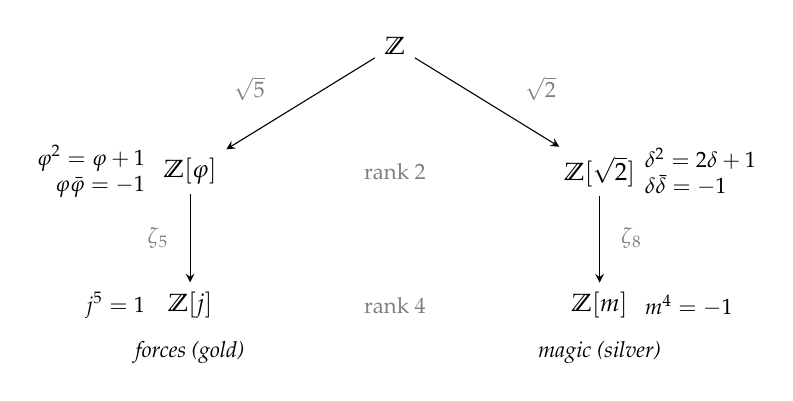
\begin{tikzpicture}[
  every node/.style={font=\small},
  arrow/.style={->, >=stealth, thin}
]
  \node (Z) at (0,4) {$\mathbb{Z}$};
  \node (Zphi) at (-2.6,2.4) {$\mathbb{Z}[\ph]$};
  \node (Zd) at (2.6,2.4) {$\mathbb{Z}[\sqrt{2}]$};
  \node (Zj) at (-2.6,0.7) {$\mathbb{Z}[j]$};
  \node (Zm) at (2.6,0.7) {$\mathbb{Z}[m]$};

  % edge labels: what is adjoined
  \node[font=\footnotesize, gray] at (-1.85,3.45) {$\sqrt{5}$};
  \node[font=\footnotesize, gray] at (1.85,3.45) {$\sqrt{2}$};
  \node[font=\footnotesize, gray, anchor=east] at (-2.75,1.55) {$\zeta_5$};
  \node[font=\footnotesize, gray, anchor=west] at (2.75,1.55) {$\zeta_8$};

  % node relations: metallic law + norm = -1
  \node[font=\footnotesize, anchor=east, align=right] at (-3.05,2.4) {$\ph^2 = \ph + 1$\\$\ph\bar\ph = -1$};
  \node[font=\footnotesize, anchor=west, align=left] at (3.05,2.4) {$\delta^2 = 2\delta + 1$\\$\delta\bar\delta = -1$};
  \node[font=\footnotesize, anchor=east] at (-3.05,0.7) {$j^5 = 1$};
  \node[font=\footnotesize, anchor=west] at (3.05,0.7) {$m^4 = -1$};

  % rank labels
  \node[font=\footnotesize, gray] at (0,2.4) {rank 2};
  \node[font=\footnotesize, gray] at (0,0.7) {rank 4};

  \draw[arrow] (Z) -- (Zphi);
  \draw[arrow] (Z) -- (Zd);
  \draw[arrow] (Zphi) -- (Zj);
  \draw[arrow] (Zd) -- (Zm);

  \node[font=\footnotesize\itshape] at (-2.6,0.1) {forces (gold)};
  \node[font=\footnotesize\itshape] at (2.6,0.1) {magic (silver)};
\end{tikzpicture}
\end{center}

\vspace{0.3em}

Two branches from $\mathbb{Z}$, perfect mirrors of each other. Each climbs through a real metallic ring to a four-dimensional cyclotomic integer ring. The gold branch passes through $\mathbb{Z}[\ph]$ (golden ratio $\ph$, $\ph^2 = \ph + 1$) to the twist numbers $\mathbb{Z}[j] = \mathbb{Z}[\zeta_5]$: the prime-5 world, where the forces live. The silver branch passes through $\mathbb{Z}[\sqrt{2}]$ (silver ratio $\delta = 1 + \sqrt{2}$, $\delta^2 = 2\delta + 1$) to the magic numbers $\mathbb{Z}[m] = \mathbb{Z}[\zeta_8]$: the prime-2 world, where quantum computation lives.

The mirror is exact. Both metallic fundamental units have norm $-1$: $\ph\bar\ph = -1$ and $\delta\bar\delta = -1$, where the bar denotes the Galois conjugate. Both rings above them are CM fields, totally imaginary quadratic extensions of the totally real metallic base: $\mathbb{Q}(\sqrt{5})$ under gold, $\mathbb{Q}(\sqrt{2})$ under silver. And the top relations rhyme: $j^5 = 1$ on the gold side, $m^4 = -1$ on the silver. They are disjoint over $\mathbb{Q}$, since $\mathbb{Q}(\zeta_5) \cap \mathbb{Q}(\zeta_8) = \mathbb{Q}$. Forces on five, computation on two, meeting only at the integers.

(The magic numbers also contain the Gaussian integers $\mathbb{Z}[i]$, since $m^2 = i$; that is the route taken in the companion paper on magic numbers, where $m = \sqrt{i}$ is the $T$ gate of quantum computation. Here we follow the metallic route, to show the mirror with gold.)

% ============================ XIII ============================
\newpage
\section*{XIII. Summary}

Three equations. Three levels. One tower.

\begin{equation*}
\text{(none)} \;\longrightarrow\; \ph^2 = \ph + 1 \;\longrightarrow\; j + j^2 + j^3 + j^4 = -1
\end{equation*}

\begin{equation*}
\mathbb{Z} \;\longrightarrow\; \TTr \;\longrightarrow\; \TT
\end{equation*}

\begin{equation*}
1\text{D} \;\longrightarrow\; 2\text{D} \;\longrightarrow\; 4\text{D}
\end{equation*}

\vspace{0.5em}

\begin{center}
\textit{$i$ extends the integers to a plane.}\\[0.3em]
\textit{$j$ extends the integers to a space.}\\[0.3em]
\textit{The golden ratio is the midpoint.}
\end{center}

\vspace{1.5em}

% ============================ NOTATION ============================
\section*{Notation}

\renewcommand{\arraystretch}{1.4}
\begin{tabularx}{\textwidth}{c l L}
\toprule
\textit{Symbol} & \textit{Name} & \textit{Definition} \\
\midrule
$j$ & Twist unit & $j + j^2 + j^3 + j^4 = -1$,\; $j \notin \mathbb{R}$ \\[0.3em]
$\TT$ & Twist numbers & $\mathbb{Z}[j] = \{a + bj + cj^2 + dj^3\}$ \\[0.3em]
$\TTr$ & Real twist numbers & $\mathbb{Z}[\ph] = \{a + b\ph\}$ \\[0.3em]
$J$ & Distinguished unit & $1 + j^2$,\; $N(J) = 1$,\; $|J| = 1/\ph$ (std.\ embedding) \\[0.3em]
$\ph$ & Golden ratio & $-(j^2 + j^3) = (1+\sqrt{5})/2$ \\[0.3em]
$1/\ph$ & Inverse golden ratio & $j + j^4 = (\sqrt{5}-1)/2$ \\[0.3em]
$\sigma$ & Galois generator & $j \mapsto j^2$,\; order 4 \\[0.3em]
$N(\alpha)$ & Algebraic norm & $\prod_{k=0}^{3} \sigma^k(\alpha) \in \mathbb{Z}$ \\[0.3em]
$M_j$ & Generator matrix & Companion of $\Phi_5$,\; entries $\{-1,0,1\}$ \\[0.3em]
$D_J$ & Phase motor & $M_j^2 = M_J - I$,\; entries $\{-1,0,1\}$,\; period 5 \\[0.3em]
$M_J$ & $J$ matrix & $I + D_J$,\; entries $\{-1,0,1\}$,\; $\det = 1$ \\[0.3em]
$R$ & Regulator & $\ln\ph$ for $\TTr$;\; $2\ln\ph$ for $\TT$ \\
\bottomrule
\end{tabularx}

% ============================ FINAL PAGE ============================
\newpage

\section*{References}

\begin{enumerate}[leftmargin=2em,itemsep=0.1em]
\item L.\ C.\ Washington, \textit{Introduction to Cyclotomic Fields}, 2nd ed., Springer, 1997.
\item D.\ A.\ Marcus, \textit{Number Fields}, Springer, 1977.
\item J.\ Neukirch, \textit{Algebraic Number Theory}, Springer, 1999.
\end{enumerate}

\vspace{1.5em}

% ============================ CLOSURE: DUAL EMBEDDING ============================
\begin{center}
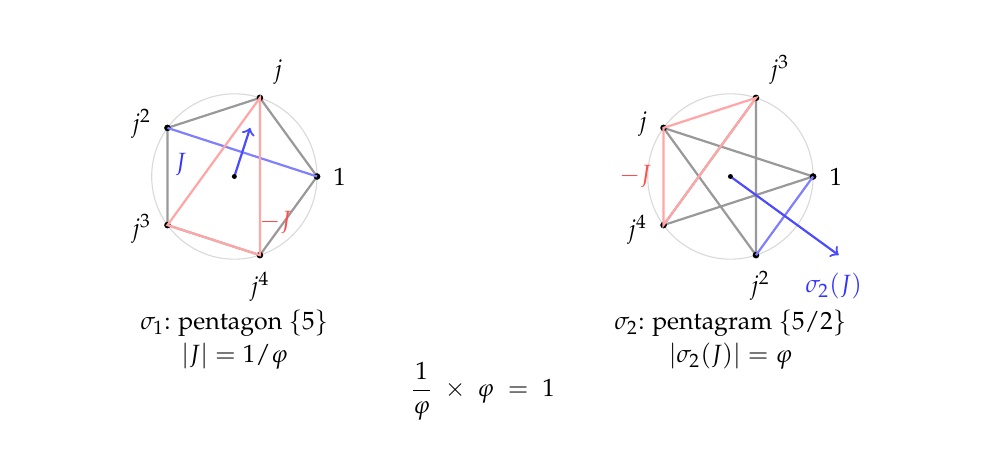
\begin{tikzpicture}[scale=1.05]

  % Bounding box padding so labels are never clipped
  \path (-5.5,-3.1) rectangle (5.8,1.8);

  % ===== LEFT: σ₁ embedding (pentagon, contracting) =====
  \begin{scope}[shift={(-3.0,0)}]
    % Unit circle
    \draw[thin, black!15] (0,0) circle (1);
    % Pentagon vertices on unit circle
    \coordinate (L0) at (0:1);     % 1
    \coordinate (L1) at (72:1);    % j
    \coordinate (L2) at (144:1);   % j²
    \coordinate (L3) at (216:1);   % j³
    \coordinate (L4) at (288:1);   % j⁴
    % Pentagon edges (regular {5})
    \draw[thick, black!40] (L0) -- (L1) -- (L2) -- (L3) -- (L4) -- cycle;
    % Dots
    \foreach \k in {0,...,4} { \fill[black] (L\k) circle (0.04); }
    % Labels - pulled slightly toward center to avoid clipping
    \node[right, font=\small] at ($(L0)+(0.08,0)$) {$1$};
    \node[above right, font=\small] at ($(L1)+(0.05,0.05)$) {$j$};
    \node[left, font=\small] at ($(L2)+(-0.08,0.05)$) {$j^2$};
    \node[left, font=\small] at ($(L3)+(-0.08,-0.05)$) {$j^3$};
    \node[below, font=\small] at ($(L4)+(0,-0.08)$) {$j^4$};
    % J partition (blue): 1 and j²
    \draw[blue!50, thick] (L0) -- (L2);
    % -J partition (red): j, j³, j⁴
    \draw[red!35, thick] (L1) -- (L3) -- (L4) -- cycle;
    \node[font=\small\bfseries, red!70] at (0.5,-0.55) {$-J$};
    % J vector (short: 1/φ ≈ 0.618)
    \draw[->, thick, blue!70] (0,0) -- (0.191, 0.588);
    \node[font=\small\bfseries, blue!80] at (-0.65, 0.15) {$J$};
    % Origin
    \fill[black] (0,0) circle (0.03);
    % Caption
    \node[below, font=\small] at (0,-1.5) {$\sigma_1$: pentagon $\{5\}$};
    \node[below, font=\small] at (0,-1.9) {$|J| = 1/\ph$};
  \end{scope}

  % ===== RIGHT: σ₂ embedding (pentagram, expanding) =====
  \begin{scope}[shift={(3.0,0)}]
    % Unit circle
    \draw[thin, black!15] (0,0) circle (1);
    \coordinate (R0) at (0:1);     % 1
    \coordinate (R1) at (144:1);   % j  (at 144°)
    \coordinate (R2) at (288:1);   % j² (at 288°)
    \coordinate (R3) at (72:1);    % j³ (at 72°)
    \coordinate (R4) at (216:1);   % j⁴ (at 216°)
    % Pentagram edges: connecting j-powers in order = {5/2}
    \draw[thick, black!40] (R0) -- (R1) -- (R2) -- (R3) -- (R4) -- cycle;
    % Dots at all 5 unit circle positions
    \foreach \a in {0,72,144,216,288} { \fill[black] (\a:1) circle (0.04); }
    % Labels
    \node[right, font=\small] at ($(R0)+(0.08,0)$) {$1$};
    \node[left, font=\small] at ($(R1)+(-0.08,0.05)$) {$j$};
    \node[below, font=\small] at ($(R2)+(0.05,-0.08)$) {$j^2$};
    \node[above right, font=\small] at ($(R3)+(0.05,0.05)$) {$j^3$};
    \node[left, font=\small] at ($(R4)+(-0.08,-0.05)$) {$j^4$};
    % J partition (blue): 1 (at 0°) and j² (at 288°)
    \draw[blue!50, thick] (R0) -- (R2);
    % -J partition (red): j (144°), j³ (72°), j⁴ (216°)
    \draw[red!35, thick] (R1) -- (R3) -- (R4) -- cycle;
    \node[font=\small\bfseries, red!70] at (-1.15, 0.0) {$-J$};
    % σ₂(J) vector (long: φ ≈ 1.618)
    \draw[->, thick, blue!70] (0,0) -- (1.309, -0.951);
    \node[below, font=\small\bfseries, blue!80] at (1.25, -1.05) {$\sigma_2(J)$};
    % Origin
    \fill[black] (0,0) circle (0.03);
    % Caption
    \node[below, font=\small] at (0,-1.5) {$\sigma_2$: pentagram $\{5/2\}$};
    \node[below, font=\small] at (0,-1.9) {$|\sigma_2(J)| = \ph$};
  \end{scope}

  % ===== Product formula =====
  \node[font=\small] at (0, -2.6) {$\displaystyle \frac{1}{\ph} \;\times\; \ph \;=\; 1$};

\end{tikzpicture}
\end{center}

\vspace{0.3em}

\begin{center}
{\small The Galois action $\sigma_2\!: j \mapsto j^2$ transforms the pentagon into its star polygon.\\[0.1em]
$J$ contracts in one embedding, expands in the other. The product of moduli is $1$.}
\end{center}

\vspace{0.6em}

\begin{center}
\textit{The sum of all nontrivial powers of $i$ is $-1$.}\\[0.2em]
\textit{The sum of all nontrivial powers of $j$ is $-1$.}\\[0.2em]
\textit{The same principle. The next dimension.}
\end{center}

\vspace{1.5em}

% ============================ DEDICATION ============================
\begin{center}
\textit{I owe this work to many;}\\[0.15em]
\textit{I owe everything to the One from whom all things begin.}

\vspace{0.4em}

\textit{The universe is mathematical. And it's beautiful.}\\[0.15em]
\textit{Always the same. Forever new.}

\vspace{0.8em}


\begin{tikzpicture}[scale=0.04]
    \draw[line width=0.8pt]
      plot[samples=200, smooth, domain=0:720]
        ({0.3*exp(0.0053*\x)*cos(\x)},
         {0.3*exp(0.0053*\x)*sin(\x)});
    \draw[line width=0.6pt, opacity=0.7]
      plot[samples=200, smooth, domain=0:720]
        ({0.3*exp(0.0053*\x)*cos(\x+144)},
         {0.3*exp(0.0053*\x)*sin(\x+144)});
    \draw[line width=0.6pt, opacity=0.7]
      plot[samples=200, smooth, domain=0:720]
        ({0.3*exp(0.0053*\x)*cos(\x+288)},
         {0.3*exp(0.0053*\x)*sin(\x+288)});
    \draw[ultra thin, opacity=0.5]
      plot[samples=180, smooth, domain=0:600]
        ({0.2*exp(0.0048*\x)*cos(\x+72)},
         {0.2*exp(0.0048*\x)*sin(\x+72)});
    \draw[ultra thin, opacity=0.5]
      plot[samples=180, smooth, domain=0:600]
        ({0.2*exp(0.0048*\x)*cos(\x+216)},
         {0.2*exp(0.0048*\x)*sin(\x+216)});
\end{tikzpicture}

\vspace{0.8em}

\textsc{A.\ M.\ Thorn}\\[0.2em]
\textit{June 2026}

\end{center}

\end{document}